\chapter[Problemas de teste]{Problemas de teste}

São vários os problemas em que se pode aplicar os algoritmos multiobjetivos e pode-se dividi-los em duas categorias: contínuos ou discretos. O comportamento e até a própria possibilidade de se aplicar o algoritmo depende dessa classificação. A fim de testar os métodos multiobjetivos, normalmente se utiliza problemas de teste, dentre os contínuos, destacam-se: SCH [], FON [], POL [], KUT [] e ZDT []. Os problemas contínuos são funções contínuas e não necessariamente representam um problema real. Os problemas discretos, por outro lado, possuem um enunciado bem definido e nem todas as soluções possíveis são válidas, ou seja, existem buracos no contradomínio das funções. Exemplos de problemas discretos comummente usados na literatura multiobjetivo são: cacheiro viajante, roteamento de veículos com janelas de tempo, problema da mochila, sequenciamento de proteínas e problemas de roteamento em redes. Neste trabalho focou-se em dois problemas discretos: o problema da mochila multiobjetivo (PMM) e o problema do roteamento multicast (PRM).

\section{Problema da mochila multiobjetivo}

O problema da mochila (PM) é um problema teórico muito conhecido na computação e geralmente utilizado para se introduzir o conceito de otimização. Apesar disso, existem problemas reais equivalentes que podem ser resolvidos com as mesmas técnicas, como o escalonamento de tarefas em um sistema operacional.

O problema da mochila consiste em arranjar um conjunto de itens em uma mochila de forma a não exceder a capacidade da mesma e ao mesmo tempo maximizar o valor (lucro) dos objetos carregados. Matematicamente, dado uma mochila de capacidade $C$ e um conjunto de itens $O$, onde cada $O_i \in O$ possui um peso $peso(O_i)$ e um lucro $lucro(O_i)$, encontrar o conjunto $S \subset O$, tal que $\sum_{o \in S} peso(o) <= C$ e $\sum_{o \in S} lucro(o)$ seja o maior possível.

Existem diversas estratégias para se resolver o problema da mochila, dentre elas as mais usadas são algoritmos gulosos e algoritmos genéticos. Uma coletânea de algoritmos gulosos para o PM são explicados, implementados e analisados em [Bracis 15].  Em [Bracis 21], um AG é proposto e se demonstra o potencial da estratégia para a resolução de problemas de otimização NP-completos com restrições. Apesar de existirem múltiplas estratégias, para se resolver o problema, os algoritmos gulosos são os mais rápidos e eficientes para resolver o PM mono-objetivo, em contra-partida, a complexidade adicionada pela versão multiobjetivo do problema inviabiliza a utilização dos mesmos, tornando os AG's e demais métodos bio-inspirados as melhores opções.

O problema da mochila multiobjetivo (PMM) é similar ao original, sua única diferença está no fato de que cada item, ao invés de possuir um único valor (lucro), é composto de múltiplos valores. No PMM, a função $lucro(O_i)$ retorna um vetor ao invés de um escalar, onde cada componente representa o valor do item $O_i$ em um dos objetivos. Por exemplo, no PMM de 3 objetivos, cada $O_i \in O$ possui um vetor tri-dimensional de lucros. O objetivo do problema passa a ser maximizar todos os lucros ao invés de um único valor.

O PMM já foi utilizado várias vezes para avaliar algoritmos multi-objetivos, podendo-se destacar os trabalhos de [SPEA] [SPEA2] [MOEA/D].

\section{Problema do roteamento multicast (PRM)}

O problema do roteamento multicast aparece na engenharia de tráfego em redes de computadores e consiste em transmitir uma mensagem multicast. Uma transmissão de rede pode ser do tipo unicast, multicast ou broadcast. Em transmissões unicast conecta-se um ponto da rede a um outro ponto qualquer, para fazer isso de forma eficiente basta encontrar o melhor caminho entre os dois pontos. As comunicações broadcast caracterizam-se pelo fato de um nó da rede (servidor) enviar o conteúdo a todos os demais, para obter as melhores rotas para trafegar os dados, basta verificar a árvore geradora de custo mínimo. As transmissões multicast desejam, a partir de um nó da rede, transmitir o conteúdo para alguns outros, o que apresenta maior complexidade, pois é necessário obter uma árvore de Steiner de custo mínimo, o que é mais difícil que calcular uma única rota ou construir a árvore geradora de custo mínimo [1-plano].

O PRM é um problema além de ser um problema prático, é muito importante, pois significaria um grande avanço na geração de rotas em redes de computadores, proporcionando uma comunicação mais rápida, menos custosa e mais confiável entre dispositivos, o que é de essencial em uma era onde a maioria das pessoas consomem informação e entretenimento pela Internet. Dado que deseja-se transmitir um conteúdo via uma rede de computadores, o problema consiste em encontrar a melhor rota possível entre a fonte de dados e o destino. Matematicamente, dado uma rede representada pelo grafo $G=(V,E)$, um nó raiz $s \in V$ (nó transmissor) e um conjunto de nós destinos $D \subset V$ (nós receptores), o PRM consiste em determinar a subárvore $T$ de $G$ enraizada em $r$ que inclui todos os vértices em $D$ e apresenta o menor custo possível. Veja o exemplo da figura \ref{fig_prm_mono}.

\begin{figure}
	\label{fig_prm_grafo}
	\caption{Exemplo de rede retirado de [1-plano]}
	\centering
	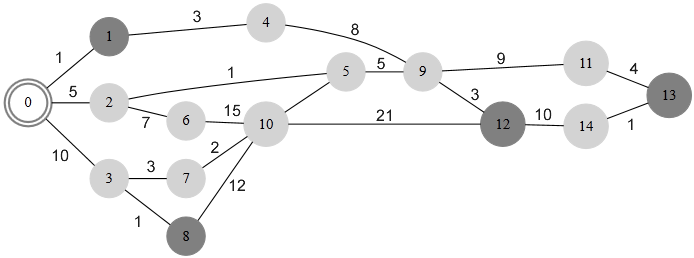
\includegraphics[width=1\textwidth]{cap_problemas/figs/prm_grafo}
\end{figure}

\begin{figure}
	\label{fig_prm_mono}
	\caption{Exemplos de árvores multicast relativos ao grafo da figura \ref{fig_prm_grafo}. Retirado do trabalho de [2-plano]}
	\centering
	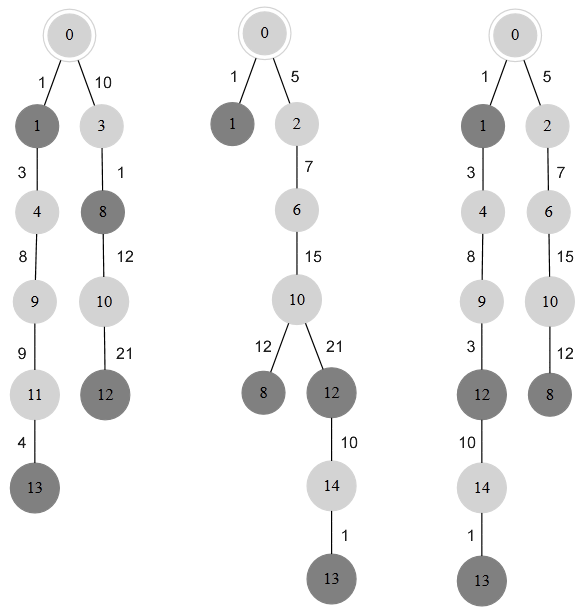
\includegraphics[width=0.8\textwidth]{cap_problemas/figs/prm_mono}
\end{figure}

Na figura \ref{fig_prm_mono} apresenta-se exemplos de árvores multicast criadas a partir do grafo mostrado na figura \ref{fig_prm_grafo} considerando a raiz ($r$) como sendo o vértice 0 e os nós destinos ($D$) igual a {1, 8, 12, 13}. O custo de cada árvore é dado pela soma dos custos de suas arestas, dentre os exemplos, a árvore mais à direita possui o menor custo total: 65.

O PRM original é proposto com apenas um objetivo a se otimizar, mas o intuito deste trabalho é utilizar uma versão mais realista do problema. A qualidade de um enlace de rede não pode ser medida através de uma única métrica, um custo genérico não é capaz de dizer se um link é bom ou ruim, características como distância, delay, capacidade de tráfego e uso do tráfego são melhores indicadores, portanto, propõe-se como objeto de estudo deste trabalho, o problema do roteamento multicast multiobjetivo. Nesta versão do problema, as árvores apresentadas como solução devem representar o melhor compromisso entre as métricas utilizadas. Veja um exemplo para a otimização de ``custo'' e ``delay'' na figura \ref{fig_prm_multi}.

\begin{figure}
	\label{fig_prm_multi}
	\caption{Exemplo de árvore multicast no PRM multiobjetivo}
	\centering
	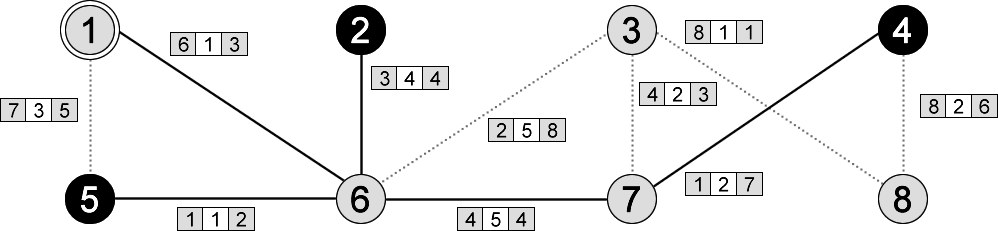
\includegraphics[width=1\textwidth]{cap_problemas/figs/prm_multi}
\end{figure}

Na figura \ref{fig_prm_multi} apresenta-se um exemplo de rede com as métricas ``custo'' (primeiro valor) e ``delay'' (segundo valor) nas arestas. As arestas em negrito representam uma árvore multicast ótima (não-dominada) para o seguinte conjunto de objetivos:

\begin{enumerate} 
	\item Minimizar custo total: soma dos valores de custo para cada aresta da árvore;
	\item Maximizar delay fim-a-fim atendidos: número de ramos da árvore em que a soma dos delays nas arestas não ultrapassa um valor $d_{max}$ pré-definido, neste caso 25. Em outras palavras, quantidade de conexões cliente-servidor que mantém limite aceitável de atraso.
\end{enumerate}

Neste trabalho considera-se até quatro valores de peso para um enlace rede: custo, delay, capacidade de tráfego e tráfego corrente, representados nas fórmulas a seguir respectivamente pelas funções: $c()$, $d()$, $z()$ e $t()$. Através dessas medidas são formulados os seguintes objetivos:

\begin{enumerate} 
	\item Custo total: soma dos valores de custo para cada aresta da árvore;
	\item Delay fim-a-fim atendidos: número de ramos da árvore em que a soma dos delays nas arestas não ultrapassa um valor $d_{max}$ pré-definido;
	\item Delay total: soma dos valore de delay para cada aresta da árvore;
	\item Delay fim-a-fim médio: média da soma dos delays em cada ramo da árvore. Em outras palavras, média do atraso em cada uma das comunicações cliente-servidor;
	\item Delay fim-a-fim máximo: maior valor para a soma de delays dentre todos os ramos da árvore;
	\item Hops count: número de vértices na árvore;
	\item Utilização máxima de enlaces: considerando todas as arestas na árvore, qual delas atinge a maior utilização de banda? Matematicamente, considerando $E$ o conjunto de arestas da árvore e $\phi$ o tamanho da mensagem, $\max_{e \in E} \frac{t(e) + \phi}{z(e)}$;
	\item Utilização média dos enlaces: média entre a utilização de banda entre todas as arestas da árvore. Similar à definição anterior.
\end{enumerate}

Afim de possibilitar diversos cenários de teste para o PRM, os objetivos acima podem ser combinados de diversas maneiras, criando vários ambientes multi-objetivos. Tais combinações são exploradas na seção de experimentos.
